
\section{Zadanie 2}
\subsection{Opis problemu}
Narysować wykres funkcji $ f(x) = e^x \ln (1 + e^{-x}) $ w co najmniej dwóch dowolnych programach do wizualizacji. Następnie policzyć granicę funkcji $ \lim_{x \to \infty} f(x) $. Porównać
wykres funkcji z policzoną granicą. Wyjaśnić zjawisko.
\subsection{Rozwiązanie}
Oto granica funkcji $ f(x) $:
$$ \lim_{x \to \infty} e^x \ln (1 + e^{-x}) = 1$$
\subsection{Wynik}
Wykresy wygenerowane za pomocą dwóch programów do wizualzacji załączone są na Rysunkach 1 i 2. Kody źródłowe programów dołączyłem do sprawozdania w osobnych plikach. \\\\
Jak widać na wykresach, w pewnym momencie funkcja zaczyna przyjmować nieoczekiwane - błędne - wartości. Głównym czynnikiem wpływającym na takie zachowanie jest operacja mnożenia bardzo dużej liczby $ e^x $ przez bardzo małą liczbę $ \ln(1 + e ^{-x}) $, bo $ \lim_{x \to \infty} \ln (1 + e^{-x}) = 0$.
\begin{figure}[!htbp]
  \centering  
  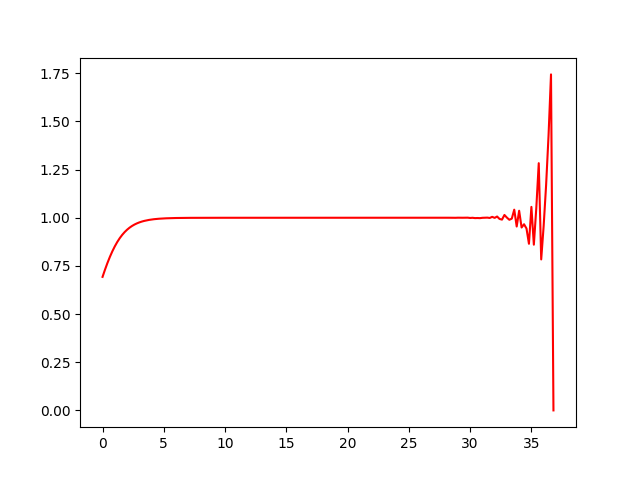
\includegraphics[totalheight=7cm]{../source/task-2/matplotlib.png}
  \caption{Wykres wygenerowany za pomocą biblioteki matplotlib w języku Python}
  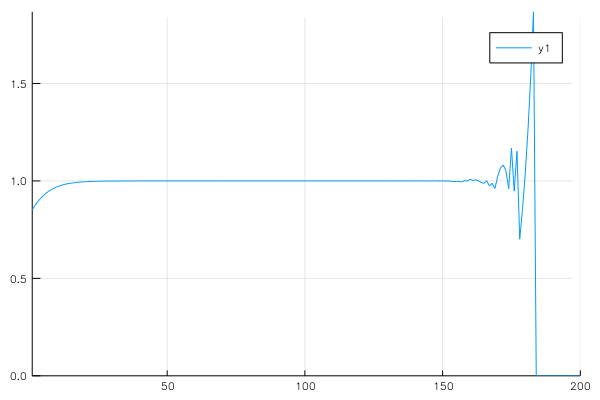
\includegraphics[totalheight=6cm]{../source/task-2/juliaplot.png}
  \caption{Wykres wygenerowany za pomocą biblioteki Plot w języku Julia}
\end{figure}
